\documentclass[aspectratio=169,11pt]{beamer}

% -----------------------------------------------------------------------------
% Self-contained presentation setup
% -----------------------------------------------------------------------------
\usepackage[T1]{fontenc}
\usepackage{lmodern}
\usepackage{amsmath,amssymb,mathtools}
\usepackage{booktabs}
\usepackage{tabularx}
\usepackage{listings}
\usepackage{tikz}
\usepackage[most]{tcolorbox}
\usepackage{appendixnumberbeamer}
\usetikzlibrary{arrows.meta,calc,decorations.pathreplacing,fit,matrix,positioning,shapes.geometric}

\usetheme{Boadilla}
\usecolortheme{seagull}
\setbeamertemplate{navigation symbols}{}
\setbeamertemplate{items}[circle]
\setbeamertemplate{enumerate items}[default]
\setbeameroption{hide notes}

\definecolor{osblue}{RGB}{28,86,145}
\definecolor{osgreen}{RGB}{36,125,91}
\definecolor{osorange}{RGB}{202,105,36}
\definecolor{osred}{RGB}{166,45,45}
\definecolor{osgray}{RGB}{74,85,104}
\setbeamercolor{structure}{fg=osblue}
\setbeamercolor{alerted text}{fg=osred}
\setbeamercolor{block title}{bg=osblue!15,fg=black}
\setbeamercolor{block body}{bg=osblue!4,fg=black}

\newcommand{\concept}[1]{\textcolor{osblue}{\textbf{#1}}}
\newcommand{\code}[1]{\texttt{#1}}
\newcommand{\smallnote}[1]{\par\vspace{0.2em}{\scriptsize\color{osgray}#1}}
\newcolumntype{C}{>{\centering\arraybackslash}X}
\newcommand{\ganttblock}[4]{%
  \filldraw[fill=#4,draw=white] (#1,.25) rectangle (#2,.95);
  \node at ({(#1+#2)/2},.60) {#3};
}
\newcommand{\ganttticks}[1]{%
  \foreach \tick in {#1}{\draw (\tick,.12)--(\tick,-.08)
    node[below,font=\scriptsize]{\tick};}
}
\newcommand{\examplemeans}[4]{%
  \begin{tcolorbox}[title=Final means (rounded to two decimals)]
    \centering
    $\overline{T}=#1\qquad\overline{W}=#2\qquad
     \overline{R}=#3\qquad\overline{S}=#4$
    \par\smallskip\scriptsize $T,W,R$: time units; $S$: dimensionless slowdown.
  \end{tcolorbox}
}

\tcbset{
  enhanced,
  boxrule=.7pt,
  arc=1.5mm,
  left=1.2mm,right=1.2mm,top=.8mm,bottom=.8mm,
  colback=osblue!3,
  colframe=osblue!60
}

\lstset{
  basicstyle=\scriptsize\ttfamily,
  keywordstyle=\color{osblue}\bfseries,
  commentstyle=\color{osgreen!80!black},
  stringstyle=\color{osred},
  numbers=left,
  numberstyle=\tiny\color{osgray},
  numbersep=5pt,
  frame=single,
  rulecolor=\color{black!20},
  backgroundcolor=\color{black!2},
  breaklines=true,
  showstringspaces=false,
  columns=fullflexible,
  keepspaces=true
}

\setbeamertemplate{footline}{%
  \leavevmode%
  \hbox{%
    \begin{beamercolorbox}[wd=.18\paperwidth,ht=2.6ex,dp=1.1ex,center]{author in head/foot}
      \insertshortauthor
    \end{beamercolorbox}%
    \begin{beamercolorbox}[wd=.64\paperwidth,ht=2.6ex,dp=1.1ex,center]{title in head/foot}
      \insertshorttitle\ifx\insertsection\empty\else\enspace---\enspace\insertsection\fi
    \end{beamercolorbox}%
    \begin{beamercolorbox}[wd=.18\paperwidth,ht=2.6ex,dp=1.1ex,center]{date in head/foot}
      \insertframenumber{} / \inserttotalframenumber
    \end{beamercolorbox}%
  }
}

\AtBeginSection[]{
  \begin{frame}[plain,noframenumbering]{Road map}
    \tableofcontents[currentsection,hideothersubsections]
  \end{frame}
}

\title[CPU Scheduling I]{CPU Scheduling Algorithms I}
\subtitle{Week 5: FCFS, SJF/SRTF, priority scheduling, and Round Robin}
\author[SDB]{SDB}
\date{Autumn 2026}

\begin{document}

\begin{frame}[plain,noframenumbering]
  \titlepage
  \vspace{-1.2em}
  \begin{center}
    \small Intermediate/graduate engineering lecture set
  \end{center}
\end{frame}

\begin{frame}{Learning outcomes}
  By the end of this lecture set, you should be able to:
  \begin{enumerate}
    \item state a scheduling model and all tie-breaking assumptions before solving it;
    \item compute completion, turnaround, waiting, response, and slowdown metrics;
    \item construct FCFS, SJF, SRTF, priority (both variants), and RR schedules;
    \item state precisely when SJF/SRTF optimality results apply;
    \item explain convoy effects, starvation, prediction error, and quantum trade-offs;
    \item incorporate idle time, context-switch cost, arrivals, and blocking correctly; and
    \item generalize size-based selection to explicit priority keys without assuming the same optimality guarantees.
  \end{enumerate}
  \begin{tcolorbox}[title=Guiding question,colback=osorange!5,colframe=osorange!70]
    Which schedule is ``best''---and best according to whose objective, information, and assumptions?
  \end{tcolorbox}
\end{frame}

\begin{frame}{Road map}
  \tableofcontents
\end{frame}

% =============================================================================
\section{Model and Evaluation Metrics}
% =============================================================================

\begin{frame}{Start with a model, not an algorithm name}
  A scheduling problem must specify:
  \begin{columns}[T,onlytextwidth]
    \column{0.49\textwidth}
      \textbf{Workload assumptions}
      \begin{itemize}
        \item one CPU or multiple/heterogeneous CPUs;
        \item arrival/release time $a_i$;
        \item CPU service/burst $b_i$;
        \item deadlines, weights, priorities;
        \item CPU-only jobs or alternating CPU/I/O bursts.
      \end{itemize}
    \column{0.47\textwidth}
      \textbf{Scheduler assumptions}
      \begin{itemize}
        \item preemptive or non-preemptive;
        \item clairvoyant or predicted service times;
        \item work-conserving or deliberate idling;
        \item context-switch/preemption cost;
        \item tie-breaking and arrival-at-boundary rules.
      \end{itemize}
  \end{columns}
  \begin{alertblock}{Without these, the answer is not unique}
    Two correct implementations can produce different Gantt charts when equal keys, simultaneous arrivals, or quantum-boundary arrivals are unspecified.
  \end{alertblock}
  \note{The classical examples use one identical CPU, independent jobs, known service times, zero overhead, and no blocking unless stated. Make students write these assumptions above every solution.}
\end{frame}

\begin{frame}{Conventions for every numerical example}
  \begin{itemize}
    \item One CPU; independent jobs with one known CPU burst each; no I/O.
    \item $P_i=(a_i,b_i)$ gives arrival and burst; priority examples add $p_i$.
    \item Time starts at zero. Dispatch/switch cost is zero unless explicitly added.
    \item FCFS arrival ties: smaller process index first. SJF/SRTF dispatch ties: earlier original arrival, then smaller process index.
    \item SRTF and preemptive priority retain the current job on an equal key; preempt only for a strictly better key.
    \item RR enqueues arrivals through the boundary before requeueing the expired job; simultaneous arrivals use process-index order.
  \end{itemize}
  \smallnote{Charts use half-open intervals $[\text{start},\text{end})$. Each example repeats its complete workload. Priority tie rules are restated in that section.}
\end{frame}

\begin{frame}{Notation and primary latency metrics}
  For job $i$:
  \[
    a_i=\text{arrival},\quad s_i=\text{first start},\quad
    c_i=\text{completion},\quad b_i=\text{total CPU service}.
  \]
  \begin{columns}[T,onlytextwidth]
    \column{0.50\textwidth}
      {\small
      \begin{align*}
        T_i &= c_i-a_i &&\text{turnaround},\\
        R_i &= s_i-a_i &&\text{first response},\\
        W_i &= T_i-b_i &&\text{CPU-only ready wait},\\
        S_i &= \frac{T_i}{b_i} &&\text{slowdown}.
      \end{align*}}
    \column{0.46\textwidth}
      \begin{alertblock}{Waiting-time caveat}
        In a general CPU/I/O workload,
        \[
          T_i=\text{CPU}+\text{ready wait}+\text{blocked time}.
        \]
        Therefore $T_i-b_i$ includes blocking and is not purely ready-queue waiting.
      \end{alertblock}
  \end{columns}
  \note{Response time is first service here. In real-time theory, response time commonly means release-to-completion. Always state the convention. Slowdown protects short jobs from looking good only in absolute units.}
\end{frame}

\begin{frame}{System-level objectives conflict}
  \small
  \begin{tabularx}{\textwidth}{@{}lXX@{}}
    \toprule
    \textbf{Objective} & \textbf{Measure} & \textbf{Potential conflict} \\
    \midrule
    throughput & completions per unit time & batching may increase response latency \\
    utilization & fraction of capacity doing defined useful work & 100\% load can create long queues \\
    mean turnaround & $\frac1n\sum_i T_i$ & can sacrifice long jobs and tail latency \\
    response & mean/percentiles of $R_i$ & frequent preemption harms locality \\
    fairness & equal/weighted service over an interval & may reduce mean completion performance \\
    deadline success & misses, tardiness, lateness & can reject or deprioritize best-effort work \\
    predictability & variance, high percentiles, bounds & conservative control may reduce average throughput \\
    energy & joules/task or performance per watt & consolidation/frequency changes latency \\
    \bottomrule
  \end{tabularx}
\end{frame}

\begin{frame}{Average metrics can hide unacceptable schedules}
  \begin{columns}[T,onlytextwidth]
    \column{0.48\textwidth}
      Report more than one mean:
      \begin{itemize}
        \item median and high-percentile latency;
        \item maximum wait over a stated interval;
        \item per-class/user/group service;
        \item slowdown for short versus long jobs;
        \item starvation/deadline violations;
        \item scheduler and context-switch overhead.
      \end{itemize}
    \column{0.48\textwidth}
      \begin{tcolorbox}[title=Example]
        Nine jobs finish immediately and one waits 100 seconds. A modest mean can coexist with an unusable tail and a fairness failure.
      \end{tcolorbox}
      \begin{alertblock}{Optimization needs a stakeholder}
        Minimizing total completion time values completed jobs equally, not users, urgency, revenue, or safety.
      \end{alertblock}
  \end{columns}
\end{frame}

\begin{frame}{Online/offline and clairvoyant/non-clairvoyant}
  \begin{columns}[T,onlytextwidth]
    \column{0.49\textwidth}
      \begin{block}{Arrival information}
        \textbf{Online}: only released jobs are known.\par
        \textbf{Offline}: the entire instance, including future arrivals, is known.
      \end{block}
      \begin{itemize}
        \item Online does not mean size-blind.
        \item Offline information can support deliberate idling.
      \end{itemize}
    \column{0.48\textwidth}
      \begin{block}{Service-time information}
        \textbf{Clairvoyant}: knows a released job's service requirement.\par
        \textbf{Non-clairvoyant}: learns through execution or uses estimates.
      \end{block}
      \begin{itemize}
        \item Exact-size SRTF can be online \emph{and} clairvoyant.
        \item Predicted sizes do not provide exact-size guarantees.
      \end{itemize}
  \end{columns}
  \begin{tcolorbox}[title=Evaluation rule]
    Do not compare a clairvoyant optimum with an online policy without acknowledging the information advantage.
  \end{tcolorbox}
\end{frame}

% =============================================================================
\section{First-Come, First-Served}
% =============================================================================

\begin{frame}{FCFS/FIFO: arrival order}
  \begin{columns}[T,onlytextwidth]
    \column{0.52\textwidth}
      \concept{Policy}: select the oldest ready job; in the classical version, run until completion or blocking.
      \begin{itemize}
        \item simple FIFO ready queue;
        \item non-preemptive among CPU bursts;
        \item deterministic given arrival/tie order;
        \item no starvation for a finite queue with finite service times;
        \item insensitive to job size or urgency.
      \end{itemize}
    \column{0.44\textwidth}
      \begin{tcolorbox}[title=Strength]
        Low policy overhead and a transparent temporal ordering.
      \end{tcolorbox}
      \begin{alertblock}{Weakness}
        A long CPU burst can delay many short or latency-sensitive jobs even when completing them first would greatly reduce total flow time.
      \end{alertblock}
  \end{columns}
\end{frame}

\begin{frame}{Convoy effect: synchronization of delays}
  \centering
  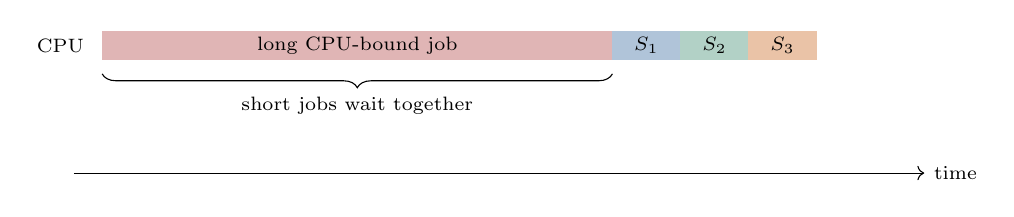
\begin{tikzpicture}[x=.72cm,y=.72cm,font=\scriptsize]
    \draw[->] (0,.4)--(15,.4) node[right]{time};
    \fill[osred!35] (.5,2.4) rectangle (9.5,2.9); \node at (5,2.65) {long CPU-bound job};
    \fill[osblue!35] (9.5,2.4) rectangle (10.7,2.9); \node at (10.1,2.65) {$S_1$};
    \fill[osgreen!35] (10.7,2.4) rectangle (11.9,2.9); \node at (11.3,2.65) {$S_2$};
    \fill[osorange!40] (11.9,2.4) rectangle (13.1,2.9); \node at (12.5,2.65) {$S_3$};
    \node[anchor=east] at (.35,2.65) {CPU};
    \draw[decorate,decoration={brace,mirror,amplitude=5pt}] (.5,2.15)--(9.5,2.15)
      node[midway,below=5pt]{short jobs wait together};
  \end{tikzpicture}
  \begin{itemize}
    \item Several short/I/O-oriented jobs accumulate behind one long CPU burst.
    \item When released, they may run briefly, issue I/O, and leave the CPU-bound job at the head again.
    \item CPU utilization need not always be low; the deeper issue is poor overlap, long response, and correlated device/CPU idle periods in some workloads.
  \end{itemize}
  \note{Avoid defining convoy effect merely as high waiting time. It is a workload synchronization effect: many tasks queue behind one long holder/job, then move as a convoy through resources.}
\end{frame}

\begin{frame}{FCFS worked example}
  Workload: $P_1=(a=0,b=8)$, $P_2=(1,4)$, $P_3=(2,9)$, $P_4=(3,5)$.
  \begin{center}
  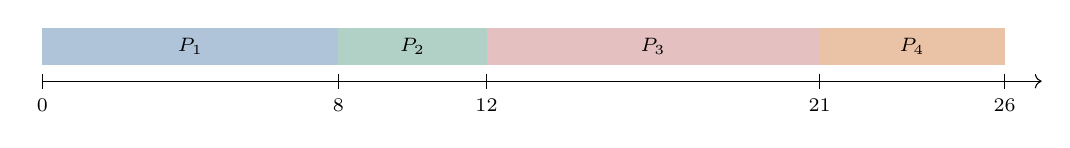
\begin{tikzpicture}[x=.47cm,y=.8cm,font=\scriptsize]
    \draw[->] (0,0)--(27,0);
    \fill[osblue!35] (0,.25) rectangle (8,.85); \node at (4,.55) {$P_1$};
    \fill[osgreen!35] (8,.25) rectangle (12,.85); \node at (10,.55) {$P_2$};
    \fill[osred!30] (12,.25) rectangle (21,.85); \node at (16.5,.55) {$P_3$};
    \fill[osorange!40] (21,.25) rectangle (26,.85); \node at (23.5,.55) {$P_4$};
    \foreach \x in {0,8,12,21,26}{\draw (\x,.12)--(\x,-.12) node[below]{\x};}
  \end{tikzpicture}
  \end{center}
  \small
  \renewcommand{\arraystretch}{1.15}
  \begin{tabularx}{\textwidth}{@{}*{6}{C}@{}}
    \toprule
    \textbf{Job} & $c_i$ & $T_i$ & $W_i$ & $R_i$ & $S_i$ \\
    \midrule
    $P_1$ & 8  & 8  & 0  & 0  & 1.00 \\
    $P_2$ & 12 & 11 & 7  & 7  & 2.75 \\
    $P_3$ & 21 & 19 & 10 & 10 & 2.11 \\
    $P_4$ & 26 & 23 & 18 & 18 & 4.60 \\
    \midrule
    mean & & 15.25 & 8.75 & 8.75 & 2.62 \\
    \bottomrule
  \end{tabularx}
\end{frame}

\begin{frame}{FCFS: six jobs, tied arrivals, and idle time}
  \small Workload $P_i=(a_i,b_i)$:
  \[
    \begin{gathered}
      P_1=(1,8),\quad P_2=(2,5),\quad P_3=(3,2),\\
      P_4=(5,1),\quad P_5=(5,3),\quad P_6=(24,2).
    \end{gathered}
  \]
  Zero overhead; no I/O; at the tied arrival, $P_4$ precedes $P_5$.
  \begin{center}
  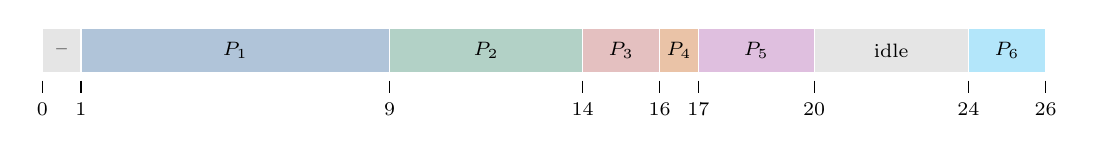
\begin{tikzpicture}[x=.49cm,y=.8cm,font=\scriptsize]
    \ganttblock{0}{1}{--}{black!10}
    \ganttblock{1}{9}{$P_1$}{osblue!35}
    \ganttblock{9}{14}{$P_2$}{osgreen!35}
    \ganttblock{14}{16}{$P_3$}{osred!30}
    \ganttblock{16}{17}{$P_4$}{osorange!40}
    \ganttblock{17}{20}{$P_5$}{violet!25}
    \ganttblock{20}{24}{idle}{black!10}
    \ganttblock{24}{26}{$P_6$}{cyan!30}
    \ganttticks{0,1,9,14,16,17,20,24,26}
  \end{tikzpicture}
  \end{center}
  \smallnote{Gray intervals denote an idle CPU, including $[0,1)$.}
  \examplemeans{10.33}{6.83}{6.83}{4.65}
  \note{The late arrival does not exist in the ready queue before time 24. Short P4 waits behind P2 and P3; simultaneous arrivals are ordered by process index.}
\end{frame}

\begin{frame}{Idle intervals must appear in the schedule}
  Jobs: $A=(a=3,b=2)$, $B=(a=8,b=1)$.
  \begin{center}
  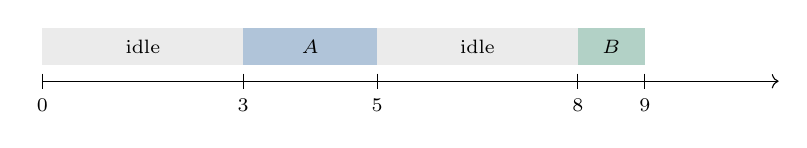
\begin{tikzpicture}[x=.85cm,y=.8cm,font=\scriptsize]
    \draw[->] (0,0)--(11,0);
    \fill[black!8] (0,.25) rectangle (3,.85); \node at (1.5,.55) {idle};
    \fill[osblue!35] (3,.25) rectangle (5,.85); \node at (4,.55) {$A$};
    \fill[black!8] (5,.25) rectangle (8,.85); \node at (6.5,.55) {idle};
    \fill[osgreen!35] (8,.25) rectangle (9,.85); \node at (8.5,.55) {$B$};
    \foreach \x in {0,3,5,8,9}{\draw (\x,.12)--(\x,-.12) node[below]{\x};}
  \end{tikzpicture}
  \end{center}
  \begin{itemize}
    \item A work-conserving scheduler idles only when no eligible job is ready.
    \item Omitting idle time changes completion and response calculations.
    \item Non-work-conserving schedules can intentionally idle for energy, reservations, or future high-value/deadline work; FCFS normally does not.
  \end{itemize}
\end{frame}

% =============================================================================
\section{Shortest-Job and Shortest-Remaining-Time}
% =============================================================================

\begin{frame}{SJF and SRTF policies}
  \begin{columns}[T,onlytextwidth]
    \column{0.49\textwidth}
      \begin{block}{Non-preemptive SJF/SPT}
        When the CPU becomes free, select the ready job with the smallest predicted/known service time; run its burst to completion or block.
      \end{block}
    \column{0.48\textwidth}
      \begin{block}{Preemptive SRTF/SRPT}
        Always run the available job with the least remaining service; a shorter arrival can preempt the current job.
      \end{block}
  \end{columns}
  \begin{itemize}
    \item Both privilege short jobs and can starve long jobs under a continuing short-job stream.
    \item Exact remaining service is normally unavailable; prediction or application declarations are required.
    \item Preemption improves the clairvoyant objective but adds switch/locality costs ignored by the ideal model.
  \end{itemize}
\end{frame}

\begin{frame}{What exactly is SJF optimal for?}
  \begin{alertblock}{Precise statement}
    For jobs available together on one identical machine, with known processing times, no preemption, and no overhead, ordering by nondecreasing processing time minimizes $\sum_i c_i$ and therefore mean completion/turnaround time.
  \end{alertblock}
  \begin{itemize}
    \item With release times, unknown sizes, weights, deadlines, blocking, or multiple CPUs, the statement requires modification and may be false.
    \item If deliberate idling is allowed and future arrivals are known, immediately running the shortest currently ready job need not be globally optimal.
    \item SRTF/SRPT provides a corresponding preemptive optimum for total flow time under its ideal single-machine clairvoyant assumptions.
  \end{itemize}
  \note{SJF also minimizes average waiting in the simultaneous-arrival CPU-only model because total service is fixed and waiting differs from completion by constants. Avoid saying it minimizes every response or tail metric.}
\end{frame}

\begin{frame}{Exchange proof for SJF optimality}
  Consider adjacent jobs $i$ then $j$ beginning at time $t$, with $b_i>b_j$.
  \begin{columns}[T,onlytextwidth]
    \column{0.48\textwidth}
      Original order $i,j$ contributes
      \[
        (t+b_i)+(t+b_i+b_j)
        =2t+2b_i+b_j.
      \]
    \column{0.48\textwidth}
      Swapped order $j,i$ contributes
      \[
        (t+b_j)+(t+b_j+b_i)
        =2t+2b_j+b_i.
      \]
  \end{columns}
  Difference:
  \[
    (2t+2b_i+b_j)-(2t+2b_j+b_i)=b_i-b_j>0.
  \]
  Thus swapping an inversion reduces total completion time. Repeatedly remove inversions to obtain shortest-processing-time order.
  \begin{tcolorbox}[title=Proof boundary]
    The argument assumes both jobs are available at $t$, their processing times are known, and swapping does not affect other constraints.
  \end{tcolorbox}
  \note{This is a local exchange argument. It is valuable because it makes assumptions visible and generalizes to many scheduling proofs.}
\end{frame}

\begin{frame}{Non-preemptive SJF worked example}
  Workload $(a_i,b_i)$: $P_1=(0,8)$, $P_2=(1,4)$, $P_3=(2,9)$, $P_4=(3,5)$.
  \begin{center}
  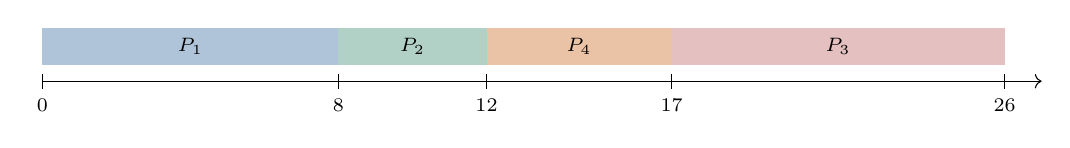
\begin{tikzpicture}[x=.47cm,y=.8cm,font=\scriptsize]
    \draw[->] (0,0)--(27,0);
    \fill[osblue!35] (0,.25) rectangle (8,.85); \node at (4,.55) {$P_1$};
    \fill[osgreen!35] (8,.25) rectangle (12,.85); \node at (10,.55) {$P_2$};
    \fill[osorange!40] (12,.25) rectangle (17,.85); \node at (14.5,.55) {$P_4$};
    \fill[osred!30] (17,.25) rectangle (26,.85); \node at (21.5,.55) {$P_3$};
    \foreach \x in {0,8,12,17,26}{\draw (\x,.12)--(\x,-.12) node[below]{\x};}
  \end{tikzpicture}
  \end{center}
  \small
  \renewcommand{\arraystretch}{1.15}
  \begin{tabularx}{\textwidth}{@{}*{5}{C}@{}}
    \toprule
    \textbf{Job} & $c_i$ & $T_i$ & $W_i$ & $R_i$ \\
    \midrule
    $P_1$ & 8  & 8  & 0  & 0 \\
    $P_2$ & 12 & 11 & 7  & 7 \\
    $P_3$ & 26 & 24 & 15 & 15 \\
    $P_4$ & 17 & 14 & 9  & 9 \\
    \midrule
    mean & & 14.25 & 7.75 & 7.75 \\
    \bottomrule
  \end{tabularx}
  \smallnote{At $t=0$, only $P_1$ is available. Non-preemptive SJF cannot replace it when shorter jobs arrive.}
\end{frame}

\begin{frame}{SJF: six jobs and non-preemptive choices}
  \small Workload $P_i=(a_i,b_i)$:
  \[
    \begin{gathered}
      P_1=(1,8),\quad P_2=(2,5),\quad P_3=(3,2),\\
      P_4=(5,1),\quad P_5=(5,3),\quad P_6=(24,2).
    \end{gathered}
  \]
  Zero overhead; no I/O; choose shortest only when the CPU becomes free.
  \begin{center}
  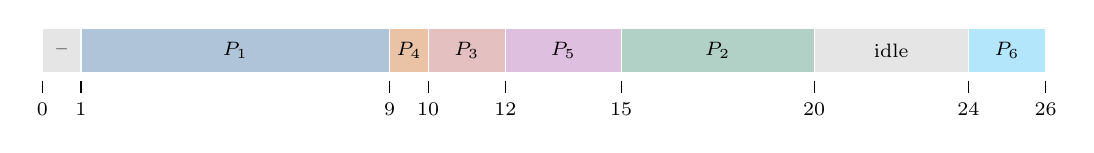
\begin{tikzpicture}[x=.49cm,y=.8cm,font=\scriptsize]
    \ganttblock{0}{1}{--}{black!10}
    \ganttblock{1}{9}{$P_1$}{osblue!35}
    \ganttblock{9}{10}{$P_4$}{osorange!40}
    \ganttblock{10}{12}{$P_3$}{osred!30}
    \ganttblock{12}{15}{$P_5$}{violet!25}
    \ganttblock{15}{20}{$P_2$}{osgreen!35}
    \ganttblock{20}{24}{idle}{black!10}
    \ganttblock{24}{26}{$P_6$}{cyan!30}
    \ganttticks{0,1,9,10,12,15,20,24,26}
  \end{tikzpicture}
  \end{center}
  \smallnote{Gray intervals denote an idle CPU, including $[0,1)$.}
  \examplemeans{8.67}{5.17}{5.17}{3.07}
  \note{At time 1 only P1 is ready. Selecting a later-arriving short job before P1 would violate work conservation. At time 9 compare only released, unfinished jobs.}
\end{frame}

\begin{frame}{SRTF worked example}
  Workload $(a_i,b_i)$: $P_1=(0,8)$, $P_2=(1,4)$, $P_3=(2,9)$, $P_4=(3,5)$.
  \begin{center}
  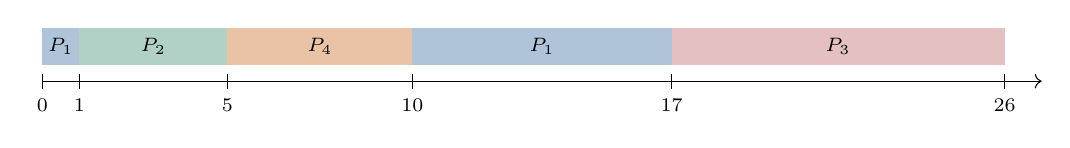
\begin{tikzpicture}[x=.47cm,y=.8cm,font=\scriptsize]
    \draw[->] (0,0)--(27,0);
    \fill[osblue!35] (0,.25) rectangle (1,.85); \node at (.5,.55) {$P_1$};
    \fill[osgreen!35] (1,.25) rectangle (5,.85); \node at (3,.55) {$P_2$};
    \fill[osorange!40] (5,.25) rectangle (10,.85); \node at (7.5,.55) {$P_4$};
    \fill[osblue!35] (10,.25) rectangle (17,.85); \node at (13.5,.55) {$P_1$};
    \fill[osred!30] (17,.25) rectangle (26,.85); \node at (21.5,.55) {$P_3$};
    \foreach \x in {0,1,5,10,17,26}{\draw (\x,.12)--(\x,-.12) node[below]{\x};}
  \end{tikzpicture}
  \end{center}
  \small
  \renewcommand{\arraystretch}{1.15}
  \begin{tabularx}{\textwidth}{@{}*{5}{C}@{}}
    \toprule
    \textbf{Job} & $c_i$ & $T_i$ & $W_i$ & $R_i$ \\
    \midrule
    $P_1$ & 17 & 17 & 9  & 0 \\
    $P_2$ & 5  & 4  & 0  & 0 \\
    $P_3$ & 26 & 24 & 15 & 15 \\
    $P_4$ & 10 & 7  & 2  & 2 \\
    \midrule
    mean & & 13.00 & 6.50 & 4.25 \\
    \bottomrule
  \end{tabularx}
\end{frame}

\begin{frame}{Why SRTF did not preempt at every arrival}
  \small Workload $(a_i,b_i)$: $P_1=(0,8)$, $P_2=(1,4)$, $P_3=(2,9)$, $P_4=(3,5)$.
  \par\medskip
  Track remaining service:
  \begin{itemize}
    \item $t=1$: $P_1$ has 7 remaining; $P_2$ arrives with 4, so preempt.
    \item $t=2$: $P_2$ has 3 remaining; $P_3$ arrives with 9, so keep $P_2$.
    \item $t=3$: $P_2$ has 2 remaining; $P_4$ arrives with 5, so keep $P_2$.
    \item $t=5$: among $P_1(7)$, $P_3(9)$, $P_4(5)$, select $P_4$.
  \end{itemize}
  \begin{alertblock}{Common error}
    ``A new job arrived'' is not itself a reason to preempt. Preempt only if the policy's ordering key makes the new/other job preferable after applying tie rules and switching cost assumptions.
  \end{alertblock}
\end{frame}

\begin{frame}{SRTF: nested preemptions and simultaneous arrivals}
  \small Workload $P_i=(a_i,b_i)$:
  \[
    \begin{gathered}
      P_1=(1,8),\quad P_2=(2,5),\quad P_3=(3,2),\\
      P_4=(5,1),\quad P_5=(5,3),\quad P_6=(24,2).
    \end{gathered}
  \]
  Zero overhead; no I/O; process all arrivals before the next selection.
  \begin{center}
  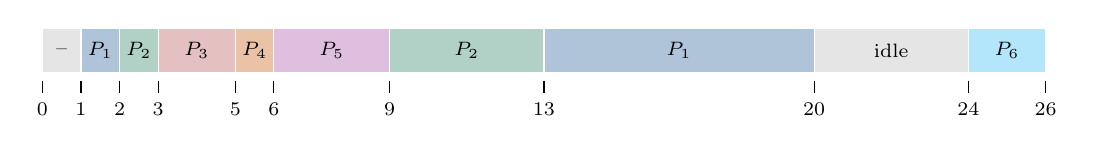
\begin{tikzpicture}[x=.49cm,y=.8cm,font=\scriptsize]
    \ganttblock{0}{1}{--}{black!10}
    \ganttblock{1}{2}{$P_1$}{osblue!35}
    \ganttblock{2}{3}{$P_2$}{osgreen!35}
    \ganttblock{3}{5}{$P_3$}{osred!30}
    \ganttblock{5}{6}{$P_4$}{osorange!40}
    \ganttblock{6}{9}{$P_5$}{violet!25}
    \ganttblock{9}{13}{$P_2$}{osgreen!35}
    \ganttblock{13}{20}{$P_1$}{osblue!35}
    \ganttblock{20}{24}{idle}{black!10}
    \ganttblock{24}{26}{$P_6$}{cyan!30}
    \ganttticks{0,1,2,3,5,6,9,13,20,24,26}
  \end{tikzpicture}
  \end{center}
  \smallnote{Gray intervals denote an idle CPU, including $[0,1)$.}
  \examplemeans{6.50}{3.00}{0.17}{1.48}
  \note{P1 is preempted at time 2 and P2 at time 3. At time 5 P3 completes as P4 and P5 arrive: select P4, then P5. Preserve P2's remaining service of 4, not its original burst of 5.}
\end{frame}

\begin{frame}{Predicting the next CPU burst}
  A classical exponential predictor is
  \[
    \tau_{n+1}=\alpha t_n+(1-\alpha)\tau_n,\qquad 0\leq\alpha\leq1,
  \]
  where $t_n$ is the observed burst and $\tau_n$ the previous prediction.
  \begin{columns}[T,onlytextwidth]
    \column{0.48\textwidth}
      Larger $\alpha$:
      \begin{itemize}
        \item reacts quickly to phase changes;
        \item increases noise sensitivity;
        \item forgets older history rapidly.
      \end{itemize}
    \column{0.48\textwidth}
      Smaller $\alpha$:
      \begin{itemize}
        \item smooths noise;
        \item adapts slowly;
        \item can lag changing workloads.
      \end{itemize}
  \end{columns}
  \begin{alertblock}{Prediction changes the policy}
    Shortest \emph{predicted} job is not clairvoyant SJF. Prediction errors can reverse priorities, cause starvation, and be gamed by strategic workloads.
  \end{alertblock}
\end{frame}

\begin{frame}{Starvation and aging}
  \begin{columns}[T,onlytextwidth]
    \column{0.50\textwidth}
      SJF/SRTF can postpone a long job indefinitely if short jobs keep arriving faster than the long job receives service.
      \begin{itemize}
        \item finite initial job sets eventually finish;
        \item open systems need an explicit liveness/fairness policy;
        \item tail latency can be poor despite an excellent mean.
      \end{itemize}
    \column{0.46\textwidth}
      \begin{tcolorbox}[title=Aging]
        Increase effective priority as waiting grows, or blend size with wait:
        \[
          \text{score}_i=f(\widehat b_i,W_i,w_i).
        \]
      \end{tcolorbox}
      \begin{alertblock}{Trade-off}
        Stronger aging protects liveness but moves the schedule away from pure shortest-job optimality.
      \end{alertblock}
  \end{columns}
\end{frame}

% =============================================================================
\section{Priority Scheduling}
% =============================================================================

\begin{frame}{From SRTF to a general priority key}
  \small SRTF succeeds for its idealized mean-flow objective by giving preference to the least remaining work. Generalize the \emph{selection mechanism}:
  \[
    \text{next}(t)\in\operatorname*{arg\,min}_{i\in\mathcal{R}(t)} k_i(t).
  \]
  Here $\mathcal{R}(t)$ contains all runnable jobs, including the current job.
  \par\medskip
  \renewcommand{\arraystretch}{1.2}
  \begin{tabularx}{\textwidth}{@{}CCC@{}}
    \toprule
    \textbf{Policy} & \textbf{Key (smaller is better)} & \textbf{Reconsider execution} \\
    \midrule
    Non-preemptive SJF & $k_i=b_i$ & when CPU becomes free \\
    SRTF & $k_i=r_i(t)$, remaining service & at arrivals/completions \\
    Fixed priority & $k_i=p_i$, assigned rank & according to preemption rule \\
    \bottomrule
  \end{tabularx}
  \begin{alertblock}{Generalizing the key does not preserve the theorem}
    An arbitrary priority ranks importance, not remaining work. It does not inherit SRTF's minimum mean-flow guarantee or promise deadlines.
  \end{alertblock}
  \note{SRTF is a dynamic size-based priority rule: its key changes with service received. Fixed-priority scheduling replaces that key with a rank independent of burst length. A priority queue is a data structure, not a synonym for a multilevel-queue policy.}
\end{frame}

\begin{frame}{Priority scheduling: two execution rules}
  \small Workload notation: $P_i=(a_i,b_i,p_i)$.
  \begin{block}{Convention for this deck}
    \textbf{Smaller number means higher priority}: $p=1$ outranks $p=2$.
    This numerical direction is a convention, not a universal OS rule.
  \end{block}
  \begin{columns}[T,onlytextwidth]
    \column{.48\textwidth}
      \begin{block}{Non-preemptive priority}
        At dispatch, choose the ready job with minimum $p_i$. It keeps the CPU until its burst ends or it blocks.
      \end{block}
    \column{.48\textwidth}
      \begin{block}{Preemptive priority}
        A newly runnable job with strictly smaller $p_i$ displaces the running job; preserve the displaced job's remaining service.
      \end{block}
  \end{columns}
  \medskip
  Equal-priority dispatch ties: \textbf{earlier original arrival}, then process index. Equal priority alone never preempts the running job. No equal-priority time slicing here.
  \note{Original arrival is retained after preemption in these CPU-only examples. This is an explicit textbook rule, not a claim about every production run queue. Real preemption also waits for a legal kernel scheduling point.}
\end{frame}

\begin{frame}{Non-preemptive priority: worked example}
  \small Workload $(a_i,b_i,p_i)$: $P_1=(0,5,3)$, $P_2=(1,3,1)$, $P_3=(2,4,2)$.
  \smallnote{Lower $p_i$ is higher priority; zero overhead; no I/O.}
  \begin{center}
  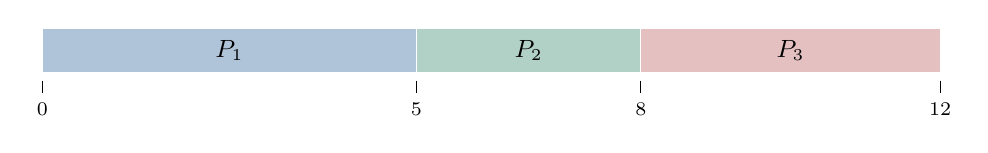
\begin{tikzpicture}[x=.95cm,y=.8cm,font=\small]
    \ganttblock{0}{5}{$P_1$}{osblue!35}
    \ganttblock{5}{8}{$P_2$}{osgreen!35}
    \ganttblock{8}{12}{$P_3$}{osred!30}
    \ganttticks{0,5,8,12}
  \end{tikzpicture}
  \end{center}
  \renewcommand{\arraystretch}{1.15}
  \begin{tabularx}{\textwidth}{@{}*{5}{C}@{}}
    \toprule
    \textbf{Job} & $c_i$ & $T_i$ & $W_i$ & $R_i$ \\
    \midrule
    $P_1$ & 5 & 5 & 0 & 0 \\
    $P_2$ & 8 & 7 & 4 & 4 \\
    $P_3$ & 12 & 10 & 6 & 6 \\
    \midrule
    mean & & 7.33 & 3.33 & 3.33 \\
    \bottomrule
  \end{tabularx}
  \smallnote{$P_2$ is highest priority but cannot displace $P_1$ at $t=1$. Priority is consulted only at dispatch.}
\end{frame}

\begin{frame}{Preemptive priority: worked example}
  \small Workload $(a_i,b_i,p_i)$: $P_1=(0,5,3)$, $P_2=(1,3,1)$, $P_3=(2,4,2)$.
  \smallnote{Lower $p_i$ is higher priority; zero overhead; no I/O.}
  \begin{center}
  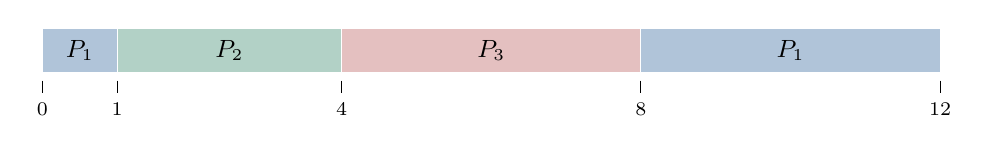
\begin{tikzpicture}[x=.95cm,y=.8cm,font=\small]
    \ganttblock{0}{1}{$P_1$}{osblue!35}
    \ganttblock{1}{4}{$P_2$}{osgreen!35}
    \ganttblock{4}{8}{$P_3$}{osred!30}
    \ganttblock{8}{12}{$P_1$}{osblue!35}
    \ganttticks{0,1,4,8,12}
  \end{tikzpicture}
  \end{center}
  \renewcommand{\arraystretch}{1.15}
  \begin{tabularx}{\textwidth}{@{}*{5}{C}@{}}
    \toprule
    \textbf{Job} & $c_i$ & $T_i$ & $W_i$ & $R_i$ \\
    \midrule
    $P_1$ & 12 & 12 & 7 & 0 \\
    $P_2$ & 4 & 3 & 0 & 0 \\
    $P_3$ & 8 & 6 & 2 & 2 \\
    \midrule
    mean & & 7.00 & 3.00 & 0.67 \\
    \bottomrule
  \end{tabularx}
  \smallnote{At $t=1$, $P_2$ preempts $P_1$. At $t=2$, $P_3$ does not preempt $P_2$: $2$ is worse than $1$.}
\end{frame}

\begin{frame}{Non-preemptive priority: six jobs and tied ranks}
  \small Workload $P_i=(a_i,b_i,p_i)$:
  \[
    \begin{gathered}
      P_1=(1,8,4),\quad P_2=(2,5,2),\quad P_3=(3,2,2),\\
      P_4=(5,1,1),\quad P_5=(5,3,3),\quad P_6=(24,2,1).
    \end{gathered}
  \]
  Zero overhead; no I/O; smaller $p$ wins, then earlier arrival/index.
  \begin{center}
  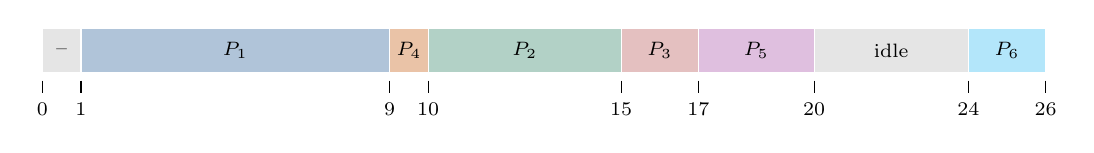
\begin{tikzpicture}[x=.49cm,y=.8cm,font=\scriptsize]
    \ganttblock{0}{1}{--}{black!10}
    \ganttblock{1}{9}{$P_1$}{osblue!35}
    \ganttblock{9}{10}{$P_4$}{osorange!40}
    \ganttblock{10}{15}{$P_2$}{osgreen!35}
    \ganttblock{15}{17}{$P_3$}{osred!30}
    \ganttblock{17}{20}{$P_5$}{violet!25}
    \ganttblock{20}{24}{idle}{black!10}
    \ganttblock{24}{26}{$P_6$}{cyan!30}
    \ganttticks{0,1,9,10,15,17,20,24,26}
  \end{tikzpicture}
  \end{center}
  \smallnote{Gray intervals denote an idle CPU, including $[0,1)$.}
  \examplemeans{9.50}{6.00}{6.00}{3.60}
  \note{P2 runs before shorter P3 because their priorities tie and P2 arrived earlier. P4 cannot displace P1 despite its superior priority. Fixed priority is not shortest-job scheduling.}
\end{frame}

\begin{frame}{Preemptive priority: interruptions and equal ranks}
  \small Workload $P_i=(a_i,b_i,p_i)$:
  \[
    \begin{gathered}
      P_1=(1,8,4),\quad P_2=(2,5,2),\quad P_3=(3,2,2),\\
      P_4=(5,1,1),\quad P_5=(5,3,3),\quad P_6=(24,2,1).
    \end{gathered}
  \]
  Zero overhead; no I/O; strictly better $p$ preempts; ties retain current job.
  \begin{center}
  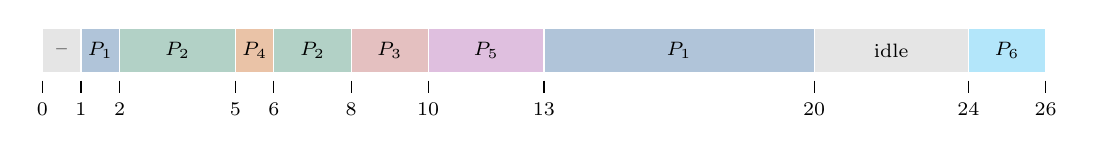
\begin{tikzpicture}[x=.49cm,y=.8cm,font=\scriptsize]
    \ganttblock{0}{1}{--}{black!10}
    \ganttblock{1}{2}{$P_1$}{osblue!35}
    \ganttblock{2}{5}{$P_2$}{osgreen!35}
    \ganttblock{5}{6}{$P_4$}{osorange!40}
    \ganttblock{6}{8}{$P_2$}{osgreen!35}
    \ganttblock{8}{10}{$P_3$}{osred!30}
    \ganttblock{10}{13}{$P_5$}{violet!25}
    \ganttblock{13}{20}{$P_1$}{osblue!35}
    \ganttblock{20}{24}{idle}{black!10}
    \ganttblock{24}{26}{$P_6$}{cyan!30}
    \ganttticks{0,1,2,5,6,8,10,13,20,24,26}
  \end{tikzpicture}
  \end{center}
  \smallnote{Equal-priority dispatch ties: original arrival, then index. Gray means idle.}
  \examplemeans{7.17}{3.67}{1.67}{1.96}
  \note{P3 arrives at time 3 with P2's priority, so it does not preempt. P4 interrupts at time 5. At time 6, P2 resumes before P3 under the original-arrival tie rule; choosing by shortest remaining time would be a different policy.}
\end{frame}

\begin{frame}{Priority: starvation, aging, and its limits}
  \small Strict fixed priority can indefinitely postpone a ready low-priority job under a continuing higher-priority workload.
  \begin{block}{One explicit aging rule (smaller is better)}
    \[
      p_i^{\mathrm{eff}}(t)=\max\!\left(p_{\min},\,
        p_i^{\mathrm{base}}-\left\lfloor\frac{w_i^{\mathrm{ready}}(t)}{\Delta}\right\rfloor\right).
    \]
    $w_i^{\mathrm{ready}}$: cumulative ready wait since the most recent dispatch, reset at dispatch. Every $\Delta$ waiting units improve the rank by one.
  \end{block}
  \begin{itemize}
    \item Reevaluate ordering when an aging threshold is crossed, not just at arrivals.
    \item Reaching the top rank is insufficient if equal-rank jobs can barge ahead or run forever; specify fair ties and finite service.
    \item Aging changes the objective: low base priority no longer means permanent subordination. It need not minimize mean turnaround.
  \end{itemize}
  \note{This is a conceptual aging policy, not a property of the fixed-priority examples. Eventual service assumes the task stays ready, finite work ahead at the top rank, no overtaking there, and a scheduler that dispatches. No universal wall-clock bound follows without bounded interference. Priority inversion instead concerns a dependency on a lower-priority resource holder; it belongs with synchronization protocols.}
\end{frame}

\begin{frame}{Priority policies compared with size-based policies}
  \small
  \renewcommand{\arraystretch}{1.2}
  \begin{tabularx}{\textwidth}{@{}XCC@{}}
    \toprule
    \textbf{Question} & \textbf{Non-preemptive priority} & \textbf{Preemptive priority} \\
    \midrule
    Higher-priority arrival? & waits for current burst & displaces lower-priority job \\
    Equal-priority arrival? & arrival/index tie at dispatch & no preemption; arrival/index tie at dispatch \\
    Needs burst prediction? & no & no \\
    Mean-flow optimality? & no general guarantee & no general guarantee \\
    Starvation risk? & sustained higher-priority work & sustained higher-priority work \\
    \bottomrule
  \end{tabularx}
  \begin{tcolorbox}[title=Keep policy and objective separate]
    SJF/SRTF rank size to improve a size-sensitive objective. Fixed priority ranks assigned importance. RR, next, instead rotates service among ready peers.
  \end{tcolorbox}
  \smallnote{Multilevel queues, feedback variants, and real-time algorithms are reserved for later lecture sets.}
\end{frame}

% =============================================================================
\section{Round Robin}
% =============================================================================

\begin{frame}{Round Robin: bounded turns in FIFO order}
  \concept{Policy}: give the head task up to quantum $q$; if still runnable after $q$, preempt and append it to the tail.
  \begin{itemize}
    \item New arrivals join the ready queue according to a specified boundary rule.
    \item A task that blocks before $q$ relinquishes the CPU; unused quantum is normally not saved.
    \item For a fixed set of $n$ continuously runnable peers and zero overhead, end-of-turn to next-start wait is at most $(n-1)q$; start-to-start spacing is at most $nq$.
    \item RR provides turn-taking, not universal fairness across weights, priorities, blocking patterns, or multicore placement.
  \end{itemize}
  \begin{tcolorbox}[title=Limiting behavior]
    $q\to\infty$ approaches FCFS. Very small $q$ approaches processor sharing in service allocation but incurs high switching and locality cost.
  \end{tcolorbox}
\end{frame}

\begin{frame}{RR queue semantics at a quantum boundary}
  Workload $(a,b)$: $A=(0,4)$, $B=(2,2)$; $q=2$, zero overhead.\par
  At $t=2$, $A$'s quantum expires exactly when $B$ arrives.
  \begin{columns}[T,onlytextwidth]
    \column{0.47\textwidth}
      \begin{block}{Rule 1}
        Process arrivals first, then append expired $A$: queue becomes $B,A$.
      \end{block}
    \column{0.47\textwidth}
      \begin{block}{Rule 2}
        Append expired $A$ first, then process arrival: queue becomes $A,B$.
      \end{block}
  \end{columns}
  \begin{alertblock}{Both can be internally consistent}
    The Gantt chart and response times differ. State the event-ordering convention before solving or simulating RR.
  \end{alertblock}
  \smallnote{This deck processes arrivals through time $t$ before requeueing the just-expired task at $t$.}
\end{frame}

\begin{frame}{RR worked example, $q=3$}
  Workload $(a_i,b_i)$: $P_1=(0,5)$, $P_2=(1,4)$, $P_3=(2,2)$.
  \begin{center}
  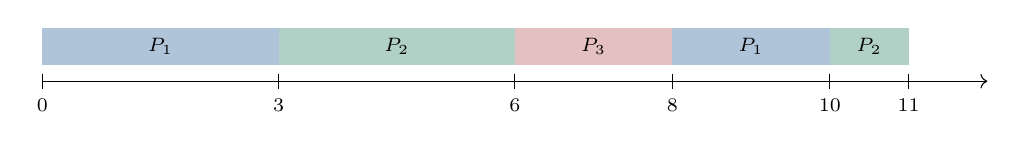
\begin{tikzpicture}[x=1.0cm,y=.8cm,font=\scriptsize]
    \draw[->] (0,0)--(12,0);
    \fill[osblue!35] (0,.25) rectangle (3,.85); \node at (1.5,.55) {$P_1$};
    \fill[osgreen!35] (3,.25) rectangle (6,.85); \node at (4.5,.55) {$P_2$};
    \fill[osred!30] (6,.25) rectangle (8,.85); \node at (7,.55) {$P_3$};
    \fill[osblue!35] (8,.25) rectangle (10,.85); \node at (9,.55) {$P_1$};
    \fill[osgreen!35] (10,.25) rectangle (11,.85); \node at (10.5,.55) {$P_2$};
    \foreach \x in {0,3,6,8,10,11}{\draw (\x,.12)--(\x,-.12) node[below]{\x};}
  \end{tikzpicture}
  \end{center}
  \small
  \renewcommand{\arraystretch}{1.15}
  \begin{tabularx}{\textwidth}{@{}*{5}{C}@{}}
    \toprule
    \textbf{Job} & $c_i$ & $T_i$ & $W_i$ & $R_i$ \\
    \midrule
    $P_1$ & 10 & 10 & 5 & 0 \\
    $P_2$ & 11 & 10 & 6 & 2 \\
    $P_3$ & 8  & 6  & 4 & 4 \\
    \midrule
    mean & & 8.67 & 5.00 & 2.00 \\
    \bottomrule
  \end{tabularx}
\end{frame}

\begin{frame}{RR state table prevents Gantt-chart mistakes}
  \small
  Workload $(a_i,b_i)$: $P_1=(0,5)$, $P_2=(1,4)$, $P_3=(2,2)$.
  \smallnote{$q=3$; zero overhead; arrivals enqueue before an expired job is requeued.}
  \par\medskip
  \renewcommand{\arraystretch}{1.15}
  \begin{tabularx}{\textwidth}{@{}cCCC@{}}
    \toprule
    \textbf{Time} & \textbf{Ready queue before dispatch} & \textbf{Run} & \textbf{Remaining afterward} \\
    \midrule
    $0$ & $[P_1]$ & $P_1:0\!\to\!3$ & $P_1=2$ \\
    $3$ & $[P_2,P_3,P_1]$ & $P_2:3\!\to\!6$ & $P_2=1$ \\
    $6$ & $[P_3,P_1,P_2]$ & $P_3:6\!\to\!8$ & completes \\
    $8$ & $[P_1,P_2]$ & $P_1:8\!\to\!10$ & completes \\
    $10$ & $[P_2]$ & $P_2:10\!\to\!11$ & completes \\
    \bottomrule
  \end{tabularx}
  \begin{tcolorbox}[title=Method]
    For RR: run until completion, blocking, or quantum expiry. Arrivals enqueue without preempting. At the boundary, enqueue arrivals before appending an unfinished expired job.
  \end{tcolorbox}
\end{frame}

\begin{frame}{RR: six jobs, boundary arrivals, and idle time}
  \small Workload $P_i=(a_i,b_i)$:
  \[
    \begin{gathered}
      P_1=(1,8),\quad P_2=(2,5),\quad P_3=(4,2),\\
      P_4=(5,1),\quad P_5=(5,3),\quad P_6=(24,2).
    \end{gathered}
  \]
  $q=3$; zero overhead; no I/O; arrivals enqueue before the expired job.
  \begin{center}
  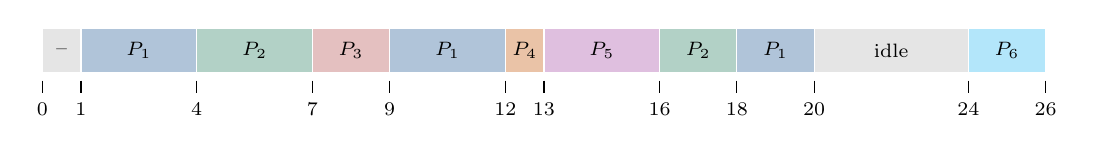
\begin{tikzpicture}[x=.49cm,y=.8cm,font=\scriptsize]
    \ganttblock{0}{1}{--}{black!10}
    \ganttblock{1}{4}{$P_1$}{osblue!35}
    \ganttblock{4}{7}{$P_2$}{osgreen!35}
    \ganttblock{7}{9}{$P_3$}{osred!30}
    \ganttblock{9}{12}{$P_1$}{osblue!35}
    \ganttblock{12}{13}{$P_4$}{osorange!40}
    \ganttblock{13}{16}{$P_5$}{violet!25}
    \ganttblock{16}{18}{$P_2$}{osgreen!35}
    \ganttblock{18}{20}{$P_1$}{osblue!35}
    \ganttblock{20}{24}{idle}{black!10}
    \ganttblock{24}{26}{$P_6$}{cyan!30}
    \ganttticks{0,1,4,7,9,12,13,16,18,20,24,26}
  \end{tikzpicture}
  \end{center}
  \smallnote{Simultaneous arrivals use process-index order. Gray means idle.}
  \examplemeans{10.17}{6.67}{3.33}{3.46}
  \note{P3 arrives exactly at time 4, before expired P1 is requeued, so P1 joins behind P2 and P3. P4 and P5 arrive at time 5 during P2's slice; neither preempts it. P5 completes exactly at the end of its quantum and must not be requeued. P6 uses only two units of its three-unit allowance.}
\end{frame}

\begin{frame}{Choosing the quantum is workload-dependent}
  \begin{columns}[T,onlytextwidth]
    \column{0.49\textwidth}
      Small $q$:
      \begin{itemize}
        \item improves turn frequency;
        \item approximates fluid sharing;
        \item raises direct switch overhead;
        \item harms cache/TLB locality;
        \item can fragment useful bursts.
      \end{itemize}
    \column{0.47\textwidth}
      Large $q$:
      \begin{itemize}
        \item improves locality/throughput;
        \item reduces scheduler overhead;
        \item approaches FCFS;
        \item increases worst-case turn wait;
        \item can hurt interactive response under load.
      \end{itemize}
  \end{columns}
  \begin{alertblock}{No universal 80\% rule}
    A common heuristic is to choose $q$ so many interactive CPU bursts finish within one slice, but the correct value depends on workload, switch cost, latency goals, CPU count, and scheduler design.
  \end{alertblock}
  \note{Modern general-purpose schedulers often do not expose one fixed global RR quantum for normal tasks. Real-time RR classes, fair schedulers, and feedback systems use different mechanisms.}
\end{frame}

\begin{frame}{Include context-switch cost in the schedule}
  \small Workload $(a_i,b_i)$: $P_1=(0,5)$, $P_2=(1,4)$, $P_3=(2,2)$; RR $q=3$.\par
  Different-task handoffs cost $s=0.2$; initial dispatch is free; no I/O.
  \begin{center}
  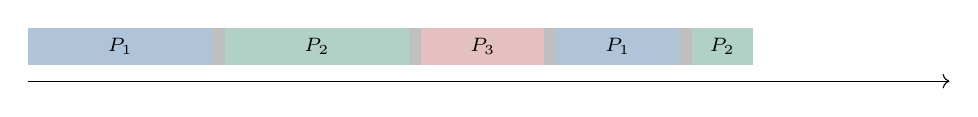
\begin{tikzpicture}[x=.78cm,y=.8cm,font=\scriptsize]
    \draw[->] (0,0)--(15,0);
    \fill[osblue!35] (0,.25) rectangle (3,.85); \node at (1.5,.55) {$P_1$};
    \fill[black!25] (3,.25) rectangle (3.2,.85);
    \fill[osgreen!35] (3.2,.25) rectangle (6.2,.85); \node at (4.7,.55) {$P_2$};
    \fill[black!25] (6.2,.25) rectangle (6.4,.85);
    \fill[osred!30] (6.4,.25) rectangle (8.4,.85); \node at (7.4,.55) {$P_3$};
    \fill[black!25] (8.4,.25) rectangle (8.6,.85);
    \fill[osblue!35] (8.6,.25) rectangle (10.6,.85); \node at (9.6,.55) {$P_1$};
    \fill[black!25] (10.6,.25) rectangle (10.8,.85);
    \fill[osgreen!35] (10.8,.25) rectangle (11.8,.85); \node at (11.3,.55) {$P_2$};
  \end{tikzpicture}
  \end{center}
  \begin{itemize}
    \item Completion times shift; recompute every metric from the cost-aware timeline.
    \item Whether idle-to-task or same-task redispatch costs $s$ must also be specified.
    \item SRTF can stop being attractive when predicted savings are smaller than preemption/warmup cost.
  \end{itemize}
\end{frame}

% =============================================================================
\section{Comparison and Deeper Insights}
% =============================================================================

\begin{frame}{FCFS, SJF, SRTF, and RR: comparison}
  \scriptsize
  \renewcommand{\arraystretch}{1.2}
  \begin{tabularx}{\textwidth}{@{}XCCCC@{}}
    \toprule
    & \textbf{FCFS} & \textbf{SJF} & \textbf{SRTF} & \textbf{RR} \\
    \midrule
    preemption & no & no & shorter remainder & quantum expiry \\
    ranking input & arrival order & burst size & remaining service & FIFO turn order \\
    ideal mean flow & may be poor & optimal if all ready together & preemptive optimum & depends on workload and $q$ \\
    first response & long-burst delays & short-job preference & short-arrival preference & bounded turn wait* \\
    starvation & none* & long jobs at risk & long jobs at risk & none* \\
    main risk & convoy & prediction error & switch cost & quantum overhead \\
    ready structure & FIFO & size-keyed heap & remainder-keyed heap & FIFO plus timer \\
    \bottomrule
  \end{tabularx}
  \smallnote{Exact positive sizes, independent CPU-only jobs, one CPU, zero overhead. *Finite ready set, finite bursts, and one service class. SJF/SRTF starvation concerns continuing arrivals.}
\end{frame}

\begin{frame}{Different objectives favor different policies}
  A scheduler can be preferable under different objectives:
  \begin{itemize}
    \item \textbf{Mean turnaround}: clairvoyant SRTF often wins in the ideal model.
    \item \textbf{Temporal transparency}: FCFS is easy to explain and reproduce.
    \item \textbf{Turn frequency/interactive sharing}: RR prevents one long CPU burst from holding the CPU indefinitely.
    \item \textbf{Tail protection}: none of these alone handles priorities, weights, or bounded starvation fully.
    \item \textbf{Production efficiency}: prediction accuracy, cache behavior, multicore placement, and overhead can reverse the textbook ranking.
  \end{itemize}
  \begin{tcolorbox}[title=No universal champion]
    An algorithm is optimal only relative to an objective, information model, constraints, and workload distribution.
  \end{tcolorbox}
\end{frame}

\begin{frame}{Competitive thinking for online schedulers}
  An online scheduler is evaluated against an offline optimum that knows the future:
  \[
    \text{competitive ratio}=\sup_{\text{workloads}}
      \frac{\text{cost of online algorithm}}{\text{cost of optimal offline algorithm}}.
  \]
  \begin{itemize}
    \item This exposes how lack of future knowledge limits guarantees.
    \item Adversarial arrivals can make simple policies perform arbitrarily badly for some objectives.
    \item Resource augmentation asks whether a slightly faster online machine can compete with an optimal baseline.
    \item Average-case traces and worst-case competitive analysis answer different questions.
  \end{itemize}
  \smallnote{A full competitive analysis is beyond this lecture, but the framework explains why clairvoyant SJF is an unfair production baseline unless its information advantage is explicit.}
\end{frame}

\begin{frame}{Multicore scheduling breaks the single timeline}
  \begin{columns}[T,onlytextwidth]
    \column{0.48\textwidth}
      Additional decisions:
      \begin{itemize}
        \item which CPU executes each thread;
        \item global versus per-CPU queues;
        \item affinity/cache/NUMA preservation;
        \item load balancing and migration;
        \item co-runner interference and SMT;
        \item heterogeneous CPU capacity/energy.
      \end{itemize}
    \column{0.48\textwidth}
      \begin{alertblock}{Proofs do not transfer automatically}
        SJF/SRTF single-machine optimality does not directly solve parallel-machine assignment, migration, precedence, or cache-affinity constraints.
      \end{alertblock}
      \begin{tcolorbox}[title=Visual model]
        Use one timeline per CPU plus migration arrows and explicit shared-resource constraints.
      \end{tcolorbox}
  \end{columns}
\end{frame}

\begin{frame}{Fairness requires a definition}
  \begin{columns}[T,onlytextwidth]
    \column{0.51\textwidth}
      Possible definitions:
      \begin{itemize}
        \item equal turns or equal CPU time per task;
        \item weighted proportional share;
        \item max-min fairness;
        \item bounded lag from an ideal fluid server;
        \item per-user/cgroup rather than per-thread fairness;
        \item priority- or deadline-constrained service.
      \end{itemize}
    \column{0.45\textwidth}
      \begin{alertblock}{RR is not automatically fair}
        Tasks that block, have different priorities, run on different CPUs, or belong to different weights receive different service. Equal quantum is only one local mechanism.
      \end{alertblock}
      \begin{tcolorbox}[title=Production view]
        Fair schedulers often approximate a weighted fluid allocation while retaining efficient discrete dispatch.
      \end{tcolorbox}
  \end{columns}
\end{frame}

\begin{frame}{Real systems combine mechanisms}
  \begin{itemize}
    \item General-purpose kernels use multiple scheduling classes/policies, priorities, weights, CPU affinity, and load balancing.
    \item Feedback mechanisms infer interactivity/CPU demand rather than know future bursts.
    \item Real-time classes use fixed-priority or deadline-oriented policies with admission/priority rules.
    \item User-space runtimes schedule tasks onto kernel threads; Grand Central Dispatch is a concurrency runtime/framework, not the kernel CPU scheduler itself.
    \item Containers/cgroups introduce hierarchical shares and quotas above per-thread decisions.
  \end{itemize}
  \begin{alertblock}{Avoid stale implementation shorthand}
    Do not equate all Linux fair scheduling with one historic data structure or all Windows behavior with a fixed version-specific number of levels. Inspect the target kernel/version.
  \end{alertblock}
  \note{The lecture's algorithms are conceptual building blocks. Production schedulers combine fairness, priority, topology, energy, and isolation, and implementation details evolve.}
\end{frame}

% =============================================================================
\section{Simulation and Verification}
% =============================================================================

\begin{frame}{Event-driven simulation structure}
  \centering
  \resizebox{.93\textwidth}{!}{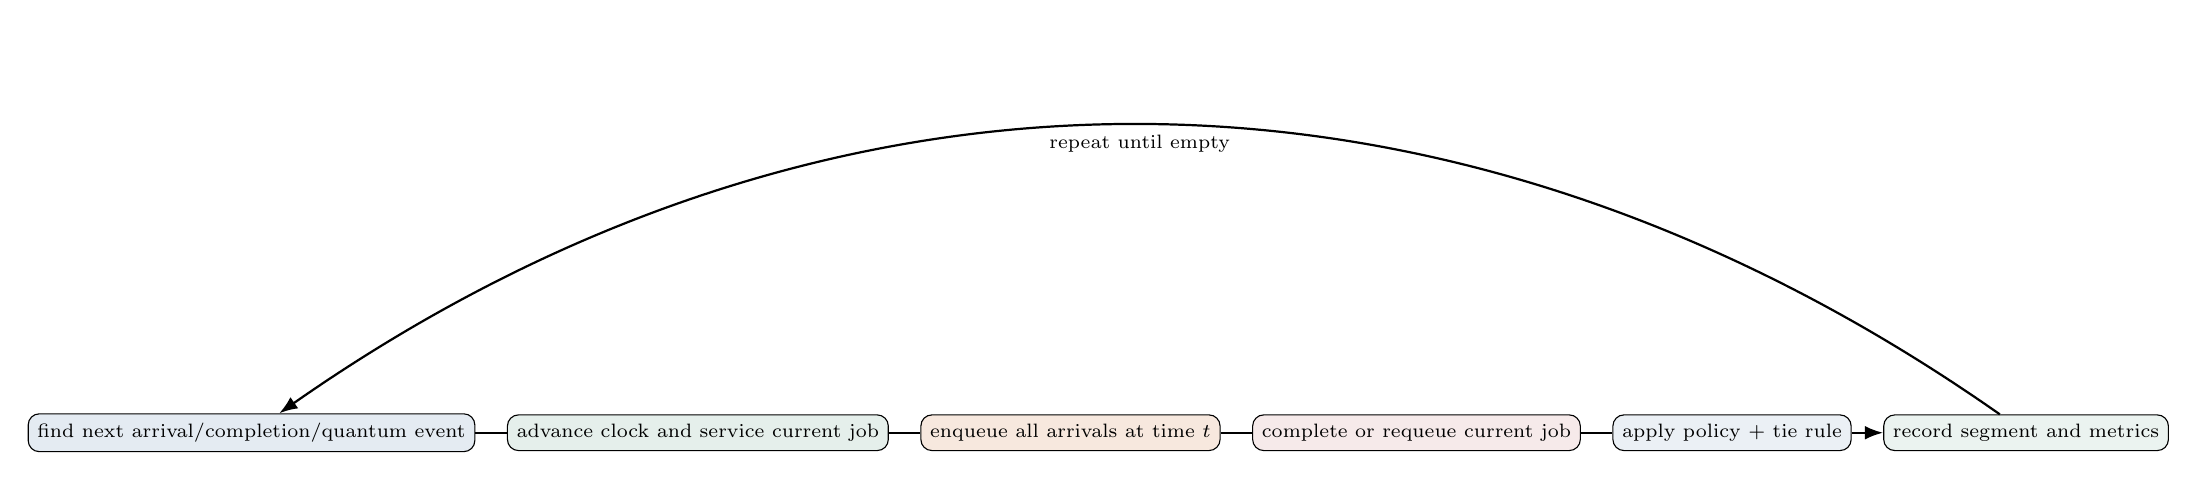
\begin{tikzpicture}[>=Latex,font=\scriptsize,node distance=4mm,every node/.style={align=center}]
    \node[draw,rounded corners,fill=osblue!12] (next) {find next arrival/completion/quantum event};
    \node[draw,rounded corners,fill=osgreen!12,right=of next] (advance) {advance clock and service current job};
    \node[draw,rounded corners,fill=osorange!15,right=of advance] (enqueue) {enqueue all arrivals at time $t$};
    \node[draw,rounded corners,fill=osred!10,right=of enqueue] (finish) {complete or requeue current job};
    \node[draw,rounded corners,fill=osblue!9,right=of finish] (select) {apply policy + tie rule};
    \node[draw,rounded corners,fill=osgreen!9,right=of select] (record) {record segment and metrics};
    \draw[->,thick] (next)--(advance)--(enqueue)--(finish)--(select)--(record);
    \draw[->,thick,bend right=35] (record) to node[below]{repeat until empty}(next);
  \end{tikzpicture}}
  \begin{itemize}
    \item Event-driven simulation avoids iterating through every time unit.
    \item Maintain remaining service, first-start time, completion time, and ready-queue order explicitly.
    \item Assert invariants: no execution before arrival, one CPU at a time, and total service equals $b_i$.
  \end{itemize}
\end{frame}

\begin{frame}[fragile]{Policy-independent metric calculation}
\begin{lstlisting}[language=Python]
for job in jobs:
    turnaround = job.completion - job.arrival
    response   = job.first_start - job.arrival
    waiting    = turnaround - job.service  # CPU-only model
    assert turnaround >= job.service
    assert response >= 0
\end{lstlisting}
  \begin{itemize}
    \item Calculate metrics from recorded timestamps, not by visually guessing the chart.
    \item For CPU/I/O traces, accumulate ready-queue residence directly rather than using $T_i-b_i$.
    \item Preserve exact rational values until presentation; round only final reported statistics.
  \end{itemize}
\end{frame}

\begin{frame}{Verification checklist for a Gantt chart}
  \begin{enumerate}
    \item Every job receives exactly its required total service.
    \item No job executes before arrival or while modeled as blocked.
    \item At each dispatch, the chosen job is optimal under the stated policy and tie rule.
    \item Every preemption is triggered by a valid policy event.
    \item Idle and context-switch intervals are explicit.
    \item Completion is the end of the final segment; first start is the beginning of the first.
    \item Mean metrics agree with per-job values and units.
  \end{enumerate}
\end{frame}

% =============================================================================
\section{Synthesis}
% =============================================================================

\begin{frame}{Misconceptions corrected}
  \small
  \begin{tabularx}{\textwidth}{@{}X@{\quad$\Rightarrow$\quad}X@{}}
    \toprule
    \textbf{Misconception} & \textbf{Precise statement} \\
    \midrule
    SJF is always optimal. & Its optimality is objective- and model-specific and assumes size knowledge. \\
    $W=T-b$ always measures ready waiting. & Only in the CPU-only model; blocking must otherwise be separated. \\
    FCFS guarantees good fairness. & It preserves arrival order but can create extreme size-dependent delay. \\
    Every arrival preempts under SRTF. & Preempt only if remaining-time ordering changes. \\
    RR eliminates starvation universally. & Only under finite equal-class runnable assumptions; priorities/weights can differ. \\
    A fixed 80\% burst heuristic gives the right quantum. & Quantum selection is workload- and system-dependent. \\
    RR is the modern desktop scheduler. & Production schedulers combine fair-share, priority, topology, and other mechanisms. \\
    Grand Central Dispatch schedules CPUs. & It schedules application work onto threads; the kernel schedules those threads. \\
    \bottomrule
  \end{tabularx}
\end{frame}

\begin{frame}{Key takeaways}
  \begin{itemize}
    \item A schedule is meaningful only with explicit workload, information, overhead, and tie assumptions.
    \item FCFS is transparent but vulnerable to convoys and poor short-job latency.
    \item SJF/SRTF optimize idealized mean flow objectives using exact service-size information that real workloads rarely provide.
    \item Explicit priority generalizes the ranking key, not SRTF's optimality guarantee.
    \item Prediction makes shortest-job policies practical but fallible and potentially unfair.
    \item RR trades locality and overhead for bounded turn frequency under a defined runnable set.
    \item Mean metrics, tail latency, slowdown, fairness, and deadlines expose different quality dimensions.
    \item Single-CPU textbook results are foundations, not complete multicore production designs.
  \end{itemize}
\end{frame}

\begin{frame}{Laboratory: build a scheduling simulator}
  Implement FCFS, SJF, SRTF, both priority variants, and RR with:
  \begin{enumerate}
    \item event-driven arrivals and explicit idle intervals;
    \item explicit priority direction, tie-breaking, and RR boundary ordering;
    \item optional dispatch/preemption cost;
    \item per-job $c_i,T_i,W_i,R_i,S_i$ and aggregate percentiles;
    \item invariant checks and a generated Gantt chart;
    \item random and adversarial workload generators.
  \end{enumerate}
  \begin{tcolorbox}[title=Experiment]
    Sweep quantum and prediction $\alpha$; compare mean flow time, $p95$ response, switch count, and starvation/maximum wait.
  \end{tcolorbox}
\end{frame}

\begin{frame}{Later lecture sets: queues, feedback, and real time}
  \begin{itemize}
    \item multilevel queues and inter-queue service policies;
    \item multilevel feedback queues and their variations;
    \item proportional-share and lottery/stride scheduling;
    \item real-time algorithms and schedulability analysis;
    \item production scheduling classes and implementation case studies.
  \end{itemize}
  \begin{tcolorbox}[title=Preparation]
    Today's core: FCFS, SJF, SRTF, non-preemptive/preemptive priority, and RR. Explain which ranking key and preemption rule each uses before adding multiple queues or deadlines.
  \end{tcolorbox}
\end{frame}

% =============================================================================
\appendix
\section{Appendix}
% =============================================================================

\begin{frame}{Knowledge check: metrics and assumptions}
  \begin{enumerate}
    \item Why is $W_i=T_i-b_i$ invalid when a task blocks for I/O?
    \item What tie rules are needed to make an RR answer reproducible?
    \item Give a workload where mean turnaround and fairness prefer different schedules.
    \item Why is response-time terminology ambiguous across scheduling fields?
    \item What information advantage does clairvoyant SRTF possess?
    \item Why must context-switch intervals be included before recomputing metrics?
  \end{enumerate}
\end{frame}

\begin{frame}{Knowledge check: algorithms}
  \begin{enumerate}
    \item State the assumptions behind non-preemptive SJF's exchange proof.
    \item Can FCFS starve a job in a finite queue with finite bursts?
    \item Why can SRTF starve a long job in an open system?
    \item When does RR approach FCFS?
    \item Does equal quantum imply equal CPU share for tasks that frequently block?
    \item Why does SRTF not preempt on every arrival?
  \end{enumerate}
  \note{Answers: simultaneous availability/known sizes/one machine/no overhead; no; endless shorter arrivals; very large q; no, blocked tasks use less CPU and other policy factors matter; only ordering-key changes justify preemption.}
\end{frame}

\begin{frame}{Knowledge check: priority is a policy, not a guarantee}
  \begin{enumerate}
    \item In what sense are SJF and SRTF special cases of priority-based selection?
    \item Why does substituting assigned ranks for remaining time lose SRTF's optimality guarantee?
    \item What happens when a higher-priority job arrives during a non-preemptive burst?
    \item Can a shorter job of equal priority preempt under this deck's priority rules?
    \item Which events should trigger reevaluation if priority changes through aging?
    \item What assumptions are needed before claiming that aging prevents starvation?
  \end{enumerate}
  \note{Keys are service size and remaining service, respectively. Arbitrary ranks need not minimize mean flow. A non-preemptive burst continues. Equal rank never preempts here, regardless of size. Aging thresholds add events. Eventual service requires finite interference and non-barging ties at the top rank, not merely a numerical boost.}
\end{frame}

\begin{frame}{Exercise: solve the common workload}
  Jobs: $P_1=(0,8)$, $P_2=(1,4)$, $P_3=(2,9)$, $P_4=(3,5)$.
  \begin{enumerate}
    \item Construct FCFS, non-preemptive SJF, and SRTF schedules.
    \item Compute $c_i,T_i,W_i,R_i,S_i$ for every job.
    \item Add a $0.5$ unit cost for each handoff to a different job.
    \item Does the relative ranking by mean turnaround change?
    \item Compare maximum wait and maximum slowdown.
  \end{enumerate}
\end{frame}

\begin{frame}{Exercise: RR boundary rules}
  Jobs: $A=(0,4)$ and $B=(2,2)$ with $q=2$.
  \begin{enumerate}
    \item Draw the schedule if arrivals at $t=2$ enqueue before expired $A$.
    \item Draw it if expired $A$ requeues before arrivals at $t=2$.
    \item Compare response and completion times.
    \item Which rule does your simulator implement, and where is it documented?
  \end{enumerate}
  \begin{tcolorbox}[title=Lesson]
    A tiny event-ordering detail changes the answer even though both implementations are recognizably Round Robin.
  \end{tcolorbox}
\end{frame}

\begin{frame}{Exercise: burst prediction}
  Let initial prediction $\tau_0=6$ and observed bursts be $t_0=2,t_1=3,t_2=12,t_3=10$.
  \begin{enumerate}
    \item Compute predictions for $\alpha=0.2$ and $\alpha=0.8$.
    \item Which reacts faster to the phase change?
    \item Compute absolute prediction error after each observation.
    \item Explain how each predictor changes SJF/SRTF ordering.
    \item Design a workload that causes repeated underprediction of a long job.
  \end{enumerate}
\end{frame}

\begin{frame}{Exercise: exchange argument with weights}
  Suppose the objective becomes weighted completion time $\sum_i w_i c_i$.
  \begin{enumerate}
    \item Compare adjacent orders $i,j$ and $j,i$.
    \item Show that the preferred order depends on $b_i/w_i$ rather than $b_i$ alone.
    \item Explain why plain SJF is no longer generally optimal.
    \item Interpret a high weight operationally: urgency, cost, user share, or business value.
  \end{enumerate}
  \note{The adjacent comparison yields Smith's rule: nondecreasing processing-time-to-weight ratio for simultaneous nonpreemptive jobs on one machine. This is an optional bridge to more advanced scheduling theory.}
\end{frame}

\begin{frame}{Further study}
  \begin{itemize}
    \item weighted completion time, Smith's rule, and scheduling with release dates;
    \item non-clairvoyant scheduling and competitive analysis;
    \item multilevel feedback queues and burst classification;
    \item proportional-share, stride, and virtual-runtime scheduling;
    \item parallel-machine scheduling, affinity, and gang scheduling;
    \item deadline scheduling, admission control, and overload behavior.
  \end{itemize}
  \begin{center}
    \Large Questions?
  \end{center}
\end{frame}

\end{document}

